\chapter{Desenvolvimento}

Esse capítulo irá discorrer sobre as metodologias e procedimentos utilizados no desenvolvimento da ferramenta.

\section{Ferramentas de desenvolvimento}

\subsection{Python}

Python \cite{pythondoc} é uma linguagem de programação de alto nível, de propósito geral e com suporte a múltiplos paradigmas de programação (orientado a objetos, imperativo, funcional), cuja sintaxe permite ao programador expressar ideias complexas em poucas linhas de código sem que ele necessite, para isso, sacrificar a clareza ou a elegância do programa. 

Sendo ela uma linguagem de código aberto, surgiu uma ampla comunidade de usuários, a qual desenvolveu diversas ferramentas para ela. Para este trabalho, as bibliotecas mais relevantes, as quais serão descritas a seguir e são todas de código aberto, são as destinadas à computação científica:

\subsection{NumPy}
NumPy é uma biblioteca que fornece funções básicas necessárias às aplicações científicas em Python. Sua principal funcionalidade é adicionar um tipo de dados versátil, juntamente com funções matemáticas, para a representação de estruturas necessárias a aplicações científicas, como matrizes e vetores \cite{numpydoc}. 

Sua sintaxe foi projetada de forma a ser similar àquela do MATLAB; dessa forma, pode-se migrar código entre as linguagens com pouca ou nenhuma dificuldade.

\subsection{SciPy}
SciPy é uma biblioteca que fornece funções para integração numérica, estatística, interpolação, otimização e processamento de sinais, entre outras empregadas na resolução de problemas matemáticos.

\subsection{SymPy}
SymPy \cite{sympydoc} é uma biblioteca cujo objetivo é a manipulação de expressões algébricas, implementando funcionalidades de um sistema algébrico computacional (\textit{computer algebra system}) na linguagem Python. 

\subsection{PyQt}
PyQt é uma biblioteca responsável pelo interfaceamento da linguagem Python com o \textit{framework} Qt, uma biblioteca desenvolvida na linguagem C++ para a construção de interfaces gráficas. Uma das suas principais vantagens, é a quase completa abstração no que diz respeito ao sistema operacional empregado: pode-se afirmar que uma interface gráfica desenvolvida em Qt irá ter aparência bastante similar em qualquer plataforma na qual ela seja executada.

As interfaces gráficas são desenhadas de forma visual utilizando-se a ferramenta \textit{Qt Designer}, a qual gera um arquivo que será convertido para código Python executável. Posteriormente, outro código define as ações (por exemplo, o que irá acontecer quando botões são clicados) e as conecta com os elementos visuais desenhados na interface.

\subsection{matplotlib}
matplotlib é uma biblioteca de plotagem de gráficos 2D, capaz de produzir diversos tipos de gráficos de alta qualidade, também podendo ser integrada à maioria das bibliotecas de interface gráfica. Seu uso pode ser feito em dois modos: em um deles, ela se comporta de forma similar às funções gráficas do MATLAB; no outro, empregado no presente trabalho, ela fornece uma interface orientada a objetos na qual gráficos são construídos.


\section{Estrutura do programa}

O programa foi estruturado conforme a seguinte estrutura de diretórios:

\dirtree{%
.1 pyfilter  \ldots{}  Diretório raiz do programa.
.2 engine    \ldots{}  Diretório com os algoritmos.
.3 filter.py \ldots{}  Estruturas de dados e funções comuns a ambos tipos de filtro.
.3 analog.py \ldots{}  Funções para projeto analógico.
.3 digital.py \ldots{} Funções para projeto digital.
.3 utils.py \ldots{} Funções diversas usadas no decorrer do programa.
.2 gui.
.3 canvas.py \ldots{} Biblioteca usada para criar gráficos na interface gráfica.
.3 gui\_analog.py \ldots{} Interface gráfica para projeto analógico.
.3 gui\_digital.py \ldots{} Interface gráfica para projeto digital.
.2 tests \ldots{} Testes (um para cada arquivo no diretório engine).
.3 test\_analog.py.
.3 test\_digital.py.
.3 test\_utils.py.
}

Dessa forma, separa-se a interface gráfica do algoritmo em si (característica desejável para facilitar o desenvolvimento: modularizando-se o código, pode-se trabalhar em uma parte dele sem que isso afete as outras).

\section{Metodologias de desenvolvimento}
\subsection{TDD (Test Driven Development)}

TDD (\textit{Test Driven Development}, na literatura em português encontrado como \textit{Desenvolvimento orientado para testes}) é uma metodologia de desenvolvimento de software que consiste em escrever testes de funcionalidade do código e, após, desenvolver código que satisfaça esses testes \cite{tdd}. 

Para adicionar-se uma nova funcionalidade ou corrigir um \textit{bug}, inicialmente escreve-se e executa-se um teste, o qual será tão específico quanto possível. Se ele executar sem erros, considera-se o desenvolvimento desta funcionalidade completo; caso contrário, o código é desenvolvido e modificado em pequenos passos (o chamado \textit{refactoring}) até que todos os testes passem com sucesso.

Dessa forma, o desenvolvedor tem maior confiança para realizar alterações em um código: se a mudança provocar falha em algum dos testes, sabe-se exatamente qual a mudança que causou o defeito; outro aspecto que torna TDD desejável é o fato dos testes documentarem a funcionalidade do código, podendo inclusive guiar o desenvolvimento deste \cite{aniche}.

Na figura \ref{fig:tdd_flow} é apresentado um fluxograma com os passos empregados.

\begin{figure}[H]
  \centering
  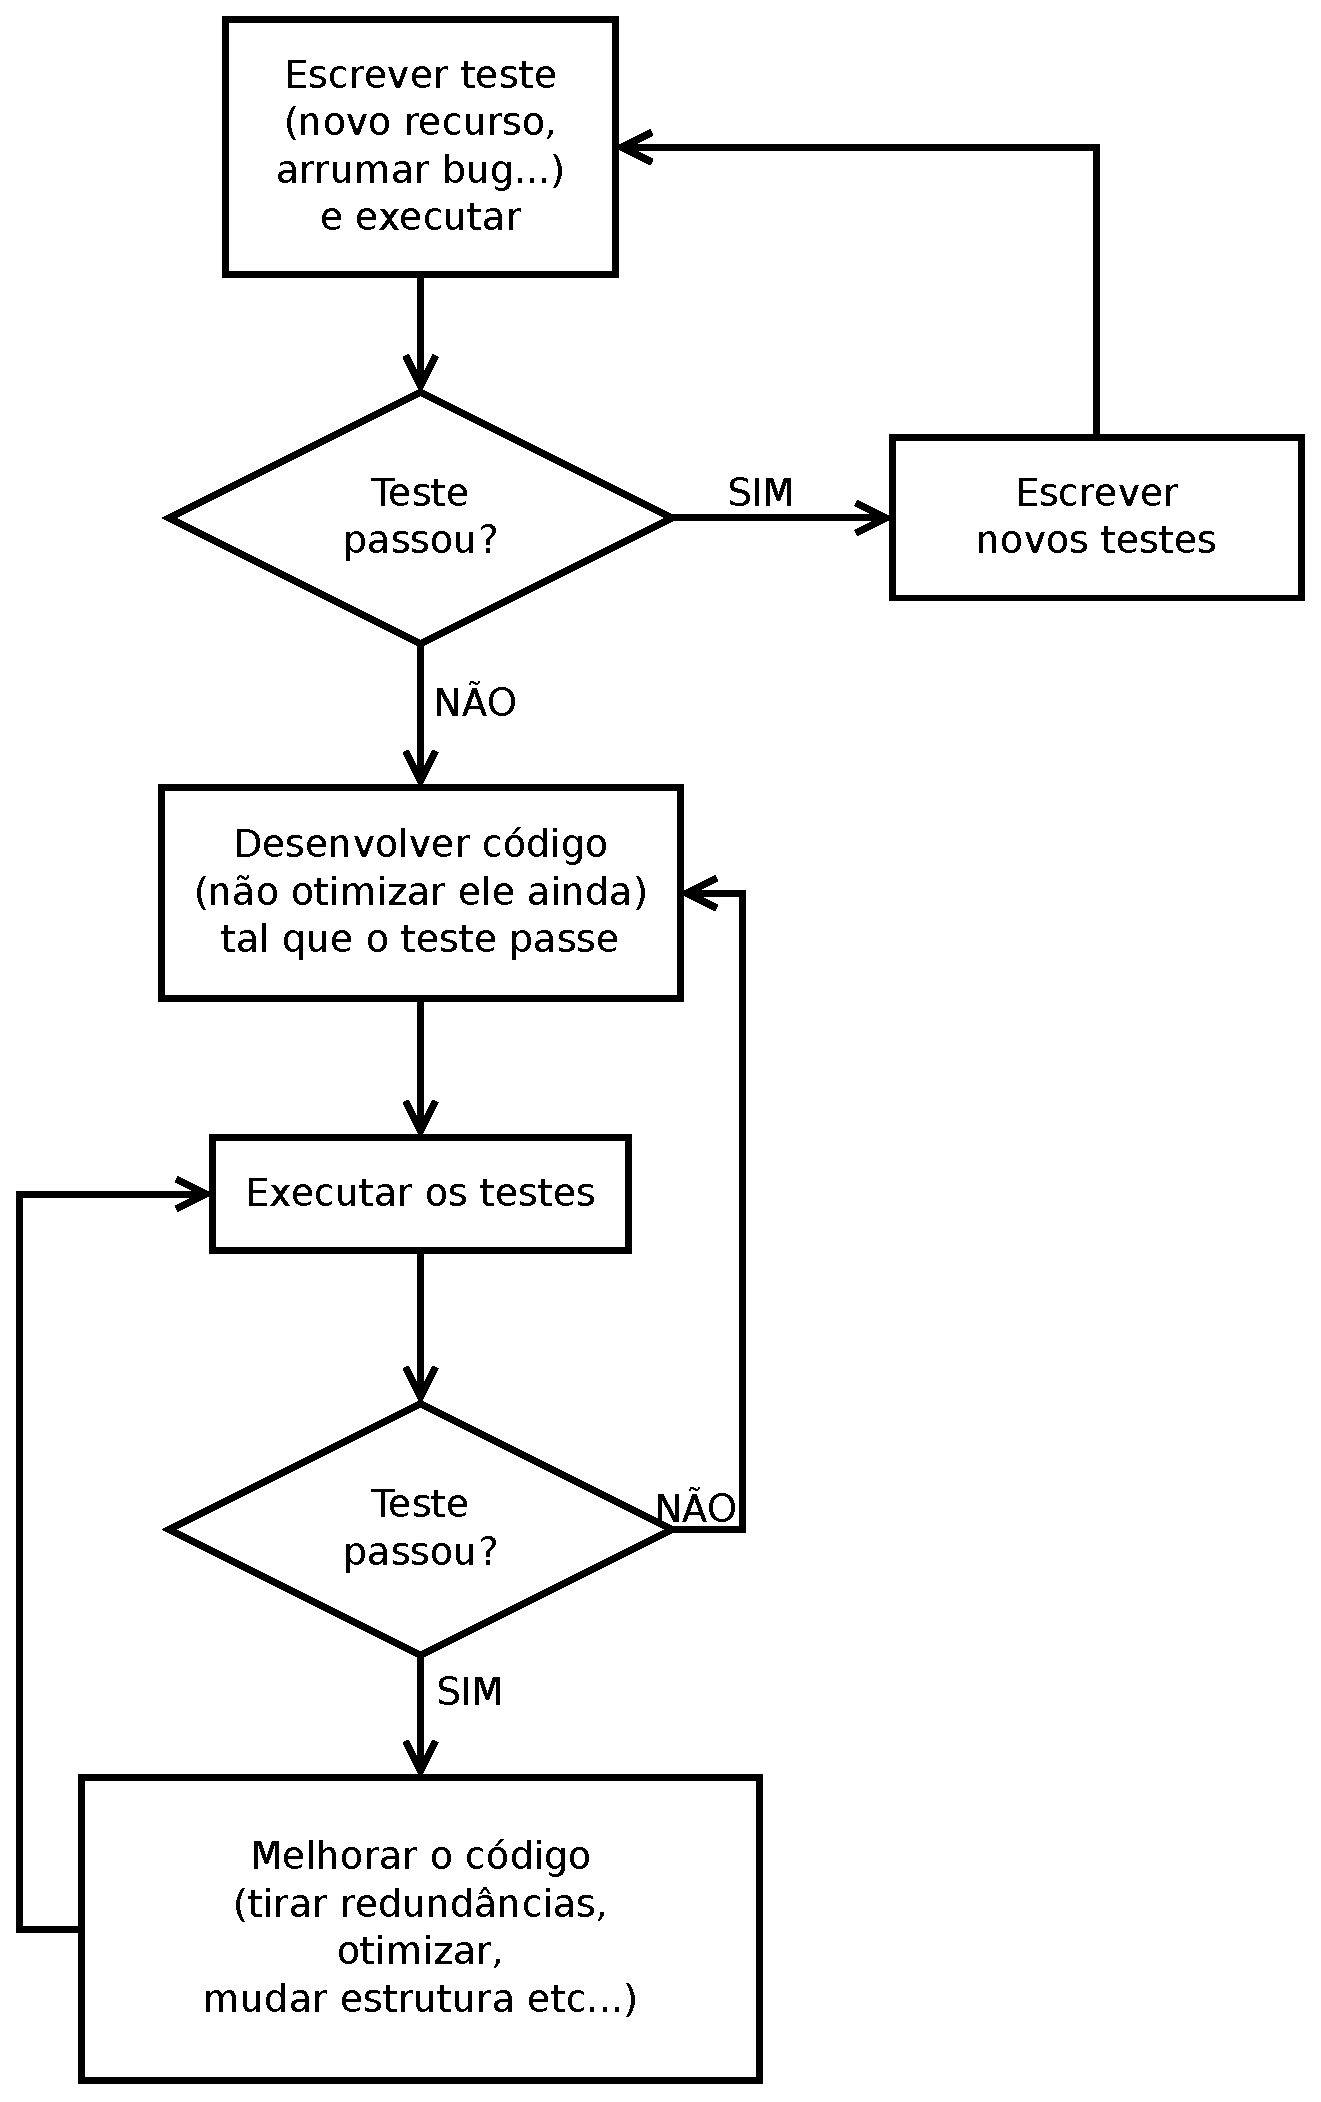
\includegraphics[scale=0.55]{images/diagrams/TDD_diagram}
  \caption{Fluxograma do desenvolvimento empregando-se TDD.}
  \label{fig:tdd_flow}
\end{figure}

Considerou-se essa metodologia adequada para o presente trabalho pois ela fornece uma maneira rápida e eficiente de testar os algoritmos e estruturas de dados, além de obrigar o desenvolvedor a pensar em termos de atender requisitos e especificações.

Neste trabalho, testes foram desenvolvidos a partir dos resultados determinados em ferramentas similares; também foram escritos testes para validar a lógica do código (por exemplo, para verificar se a detecção e tratamento de erros funcionavam adequadamente).

\subsection{Controle de versão}

Para gerenciar o desenvolvimento do \textit{software}, foi empregada a ferramenta \textit{git} para controle de versão. Dessa forma, cada modificação realizada e cada funcionalidade implementada são registradas no histórico de alterações.

Isso possibilita, entre outras conveniências, que \textit{bugs} sejam corrigidos com maior facilidade e que se tenha um histórico do desenvolvimento.

Embora não seja o caso deste trabalho, o controle de versão torna-se uma ferramenta importante e imprescindível no trabalho em equipe: cada desenvolvedor pode ter acesso ao histórico de todas as modificações feitas no código, podendo apontar exatamente o responsável por cada linha de código.

\section{Algoritmos}

No desenvolvimento do software, constatou-se que a representação dos filtros por meio de numerador e denominador poderia causar erros numéricos, especificamente para filtros de maior ordem. 

Para contornar este problema, os cálculos são realizados utilizando-se a representação ZPK (zeros/polos/ganho), isto é, são determinados vetores Z e P e um valor K tal que $G(s) = k \frac{(s - z_1) (s-z_2) \dots (s - z_n)}{(s - p_1)(s - p_2) \dots (s - p_n)}$; após, quando necessário, essa representação é convertida para uma função de transferência da forma numerador e denominador.

Para a determinação das funções de transferência dos filtros, são empregados algoritmos descritos a seguir:

\begin{itemize}
\item{\textbf{Filtros Analógicos:}} Inicialmente, é criado um filtro protótipo (isto é, um filtro com $\omega_c = 1$ rad/s) com a ordem e função de transferência desejada. 

Para determinação da ordem, são utilizadas as fórmulas clássicas descritas na fundamentação deste trabalho. Uma exceção é feita no \textit{bandstop}: emprega-se um algoritmo de zeros de função para encontrar, a partir das especificações dadas, a menor ordem que satisfaça ambas as especificações.

Posteriormente, o filtro é convertido para a frequência e tipo (passa-baixa, passa-alta, passa-faixa, rejeita-faixa) desejados utilizando-se as expressões descritas na fundamentação teórica deste trabalho.

Os filtros de Butterworth e Chebyshev são projetados por meio do posicionamento dos seus polos no plano complexo; já o filtro de Bessel é implementado diretamente, por meio de valores tabelados. Isso limita sua ordem a $N = 25$; para ordens mais altas, seria necessário expandir tais tabelas.

O filtro elíptico não possui uma representação matemática simples como os outros filtros; ele é determinado por um algoritmo iterativo de cálculo de zeros de funções, que encontra os zeros da função elíptica que atendem às especificações desejadas. Este procedimento de cálculo está descrito, juntamente com sua derivação, em \cite{orfanidis}.

\item{\textbf{Filtros Digitais FIR:}} são implementados os dois métodos vistos na revisão teórica, janelamento e Parks-McClellan.

Para o método de janelamento, as rotinas de convolução são implementadas na linguagem C para melhor desempenho - uma otimização adequada, considerando que esta basicamente envolve um grande número de somas e multiplicações, e conforme citado na introdução os processadores atuais têm instruções dedicadas para isso - e o código em Python chama essas funções quando necessário. 

Constrói-se o vetor com os valores da função janela escolhida pelo usuário (uma lista completa está disponível na documentação da biblioteca SciPy); então, é feita a convolução deste com a função de transferência projetada.

O algoritmo de Parks-McClellan, por sua vez, é uma implementação do algoritmo de Remez para aproximação de funções por meio da teoria de aproximações de Chebyshev. Podemos descrever a função erro $E$ entre o filtro ideal $D$ e o filtro real $H$, a qual será nosso objetivo minimizar, por 

\begin{equation}
E(\omega_i) = W(\omega_i) [D(e^{j \omega_i}) - H(e^{j \omega_i})] = (-1)^{i+1} \delta
\end{equation} 

onde a função $H$, que corresponde ao filtro de ordem $N$ que queremos implementar, é dada pela forma 

\begin{equation}
H(e^{j \omega}) = \sum_{k=0}^{\frac{N-1}{2}} {a_k (\cos \omega)^k}
\end{equation}

Então, precisamos encontrar coeficientes $a_k$ para $H$ que minimizem o erro. A partir das frequências especificadas e de outras estabelecidas (aleatoriamente ou calculadas nos intervalos das especificadas), executa-se um método iterativo que tenta minimizar o maior erro encontrado (o chamado método minimax). 

Neste caso, o erro aparecerá na forma de \textit{ripple}; pode-se afirmar que os filtros obtidos são \textit{equirriple}, isto é, apresentarão uma oscilação entre $-\delta$ e $\delta$ nas bandas passante e de parada.

Dessa forma, pode-se afirmar que o algoritmo de Parks-McClellan gera um filtro ótimo no sentido de minimização do \textit{ripple}, ao custo das outras características (por exemplo, nem sempre se atingem os ganhos especificados).

A dedução deste algoritmo, junto com sua análise, encontra-se disponível na literatura, por exemplo, em \cite{mcclellan_2}; uma discussão mais extensa encontra-se em \cite{souza}.

\item{\textbf{Filtros Digitais IIR:}} inicialmente é construído um filtro analógico (já com o \textit{prewarp} adequado aplicado) da topologia desejada e, após, este é discretizado empregando-se Tustin. As frequências são normalizadas na escala $0 \dots 1$, de tal forma que sua faixa vá de 0 até $f_s / 2$.

\end{itemize}

